\documentclass[french, output=paper]{langscibook}
\ChapterDOI{10.5281/zenodo.10280600}
\author{Jonas Granfeldt\orcid{}\affiliation{Université de Lund} and         Malin Ågren\orcid{}\affiliation{Université de Lund}}

\title[Le passé, le présent et l’avenir du FLE en Suède]{Le passé, le présent et l’avenir du FLE en Suède: Un bilan entre politiques linguistiques éducatives et attitudes des élèves}

\abstract{Cette étude est ancrée dans une approche transdisciplinaire de l’apprentissage des langues secondes et étrangères (\citealt{TheDouglasFirgroup2016}), composée de trois niveaux~interdépendants : un niveau \textit{macro}, caractérisé par des structures idéologiques et politiques à l'échelle de la société, un niveau \textit{méso} où se situent les établissements scolaires régis par des contraintes sociales, économiques et culturelles, et un niveau \textit{micro} défini par les apprenants eux-mêmes, leurs mécanismes neurologiques et capacités cognitives et émotionnelles. Un premier objectif de cette contribution est d’appliquer ce modèle à l’analyse du français langue étrangère (FLE) en Suède. En nous appuyant sur les données du projet TAL \citep{GranfeldtEtAl2019}, nous esquissons dans un premier temps le bilan des politiques linguistiques éducatives mises en place par des gouvernements différents après l’entrée de la Suède dans l’Union Européenne en 1995 (niveau \textit{macro}) et nous discutons leurs effets au niveau des communes et des établissements scolaires (niveau \textit{méso}). Dans un deuxième temps, nous analysons les motivations et attitudes des élèves  de FLE au collège en Suède vis-à-vis du FLE (niveau \textit{micro}). Dans l’ensemble, les données et les analyses à des niveaux différents nous permettent d’atteindre le deuxième objectif de cette contribution, à savoir une discussion du passé récent, de la situation actuelle et de l’avenir possible du FLE en Suède. 
\keywords{Français Langue Étrangère ; Langue vivante ; Suède ; Politique linguistique ; Attitudes ; Motivation}}

\IfFileExists{../localcommands.tex}{
  \addbibresource{../localbibliography.bib}
  \usepackage{langsci-optional}
\usepackage{langsci-gb4e}
\usepackage{langsci-lgr}

\usepackage{listings}
\lstset{basicstyle=\ttfamily,tabsize=2,breaklines=true}

%added by author
% \usepackage{tipa}
\usepackage{multirow}
\graphicspath{{figures/}}
\usepackage{langsci-branding}

  
\newcommand{\sent}{\enumsentence}
\newcommand{\sents}{\eenumsentence}
\let\citeasnoun\citet

\renewcommand{\lsCoverTitleFont}[1]{\sffamily\addfontfeatures{Scale=MatchUppercase}\fontsize{44pt}{16mm}\selectfont #1}
   
  %% hyphenation points for line breaks
%% Normally, automatic hyphenation in LaTeX is very good
%% If a word is mis-hyphenated, add it to this file
%%
%% add information to TeX file before \begin{document} with:
%% %% hyphenation points for line breaks
%% Normally, automatic hyphenation in LaTeX is very good
%% If a word is mis-hyphenated, add it to this file
%%
%% add information to TeX file before \begin{document} with:
%% %% hyphenation points for line breaks
%% Normally, automatic hyphenation in LaTeX is very good
%% If a word is mis-hyphenated, add it to this file
%%
%% add information to TeX file before \begin{document} with:
%% \include{localhyphenation}
\hyphenation{
affri-ca-te
affri-ca-tes
an-no-tated
com-ple-ments
com-po-si-tio-na-li-ty
non-com-po-si-tio-na-li-ty
Gon-zá-lez
out-side
Ri-chárd
se-man-tics
STREU-SLE
Tie-de-mann
}
\hyphenation{
affri-ca-te
affri-ca-tes
an-no-tated
com-ple-ments
com-po-si-tio-na-li-ty
non-com-po-si-tio-na-li-ty
Gon-zá-lez
out-side
Ri-chárd
se-man-tics
STREU-SLE
Tie-de-mann
}
\hyphenation{
affri-ca-te
affri-ca-tes
an-no-tated
com-ple-ments
com-po-si-tio-na-li-ty
non-com-po-si-tio-na-li-ty
Gon-zá-lez
out-side
Ri-chárd
se-man-tics
STREU-SLE
Tie-de-mann
} 
  \togglepaper[1]%%chapternumber
}{}

\begin{document}
\begin{otherlanguage}{french}
\lsFrenchChapterSettings{}
\SetupAffiliations{mark style=none}
\maketitle 
%\shorttitlerunninghead{}%%use this for an abridged title in the page headers



\section{Introduction}
\label{sec:granfeldt:1}

L’apprenant guidé d’une langue étrangère\footnote{Dans le domaine de l’acquisition des langues étrangères, il y a une terminologie riche pour désigner la ou les langue(s) que les apprenants sont en train d’acquérir : \textit{langue étrangère, langue seconde, deuxième langue étrangère, troisième langue étrangère, langue vivante} et \textit{langue moderne} par exemple. Dans ce texte, nous utilisons le terme \textit{langue étrangère} dans un sens général lorsque nous faisons référence à la littérature de recherche en RAL. Quand nous parlons du contexte suédois, nous alternons les termes \textit{la première langue étrangère} (toujours l’anglais en Suède) et \textit{la} \textit{deuxième langue étrangère} (souvent l’allemand, l’espagnol ou le français). Finalement, nous utilisons le terme \textit{langues vivantes} pour référer aux langues enseignées dans le contexte scolaire à partir de la 6\textsuperscript{e} classe, ce qui veut dire l’allemand, l’espagnol et le français. Il faut donc noter que dans le contexte suédois, les langues vivantes n’incluent pas l’anglais qui reste une matière indépendante et obligatoire pour les élèves pendant toute leur scolarité, ce qui n’est pas le cas des langues vivantes.}  se trouve au cœur d’un écosystème éducatif complexe (\citealt{BeaccoEtAl2005, MazièresVéronique2021}). Si, en dernier lieu, le processus d’apprentissage des langues étrangères par l’élève est largement déterminé par les ressources cognitives et psychologiques dont disposent les êtres humains, les conditions dans lesquelles ces ressources sont mobilisées et mises en œuvre sont, elles, largement déterminées par ce que nous appelons en langage ordinaire le «~contexte~». Dans le cas de l’apprentissage des langues étrangères dans une salle de classe, ce contexte est éducatif par nature et le résultat d’interactions et de pratiques au sein des institutions, contraintes à leur tour par des ressources économiques et humaines locales et, en amont, le résultat de choix politiques et idéologiques à l’échelle de la société.

A plusieurs reprises, Daniel Véronique est revenu au constat que face à cette complexité, il faudra mettre en dialogue les recherches en didactique des langues (DDL) et les recherches en acquisition des langues (RAL) (par exemple \citealt{Véronique2000recherches, Véronique2009}). Dans l’un des chapitres de clôture du volume de 2009, il discute les termes et les nombreux obstacles à un tel dialogue :

\begin{quote}
Si l’on peut poser un \textit{rapport de constitution} entre la didactique des langues et les sciences du langage, il convient d’ajouter que l’intérêt de la première discipline pour les cultures éducatives et les savoir-faire pédagogiques la conduit à entretenir \textit{de facto} des rapports avec d’autres disciplines, celles qui étudient le fait et l’idéal éducatifs par exemple. La relation que la didactique des langues étrangères entretient, en ses activités curriculaires notamment, avec les politiques éducatives et linguistiques des formations sociales où elle est mobilisée, la distingue également de maintes recherches acquisitionnelles. \hfill\hbox{(\citealt[326]{Véronique2009}, l’auteur souligne)}
\end{quote}

\begin{sloppypar}
Véronique soulève ici la transdisciplinarité nécessaire de la DDL, une conséquence de ce contexte de nature éducative dont nous avons parlé ci-dessus, comme un des obstacles majeurs derrière cette absence de dialogue entre la DDL et les RAL.\footnote{Les raisons probables derrière cette séparation sont multiples et complexes. Avec notre regard d’extérieur, il nous semble qu’elles sont d’une part internes aux disciplines concernées avec des processus généralisés de spécialisation à travers le temps et d’autre part externes aux mêmes disciplines dans le sens que les structures et les institutions responsables de ces recherches ont été séparées. Le sujet n’étant pas central ici, nous renvoyons à \citet{Hilton2021} pour une discussion récente.} Au-delà de rappeler que l’enseignement des langues étrangères se passe dans le cadre scolaire, une institution centrale au sein du système éducatif, le constat de \citet{Véronique2009} conduit aussi à souligner l’importance d’une approche théorique ouverte et holistique afin d’intégrer les concepts, les données et les interprétations de différentes disciplines. Alors qu’il y a depuis longtemps dans le domaine des RAL des approches écologiques, notamment la théorie socioculturelle de \citet{vanLier2004} et la socio-cognition d’\citet{Atkinson2011}, dont l’objectif global est de comprendre la nature située de l’acquisition des langues et l’influence du contexte sur le processus d’apprentissage, le modèle proposé du \citet{TheDouglasFirGroup2016} est avant tout transdisciplinaire dans le but de permettre le dialogue entre disciplines. Ainsi, à la base de l’approche écologique de \citet{Bronfenbrenner1979} sur le développement humain (voir aussi \citealt{Pallotti2002}), les auteurs du Douglas Fir Group développent une approche transdisciplinaire à l’étude de l’apprentissage des langues étrangères en trois niveaux~interdépendants : un niveau \textit{micro} défini par les apprenants et leurs mécanismes neurologiques, leurs capacités cognitives et émotionnelles mises en usage dans la rencontre avec l'autre dans des contextes d'actions et d'interactions multilingues spécifiques ; un niveau \textit{méso} où se situent des institutions et des communautés socioculturelles spécifiques, dont les institutions scolaires mais aussi la famille, régies par des contraintes sociales de nature économique, culturelle, idéologique et religieuse ; un niveau \textit{macro}, finalement, caractérisé par des structures idéologiques à l'échelle de la société et des institutions constituées par des croyances et des valeurs politiques, religieuses et économiques qui pèsent sur les attitudes entourant l'usage et l’apprentissage des langues dans la société en question.\footnote{Nous reviendrons à la présentation et à la discussion de ce modèle dans les sections suivantes.}
\end{sloppypar}

\begin{sloppypar}
Sur le plan empirique, il est évident qu’avec une telle modélisation riche et complexe, la question des objets d’étude pertinents se pose, surtout si l’on cherche à étudier les interdépendances inter-niveaux et leurs effets. Quelles sont les thématiques de recherche qui à la fois transcendent les trois niveaux esquissés ci-dessus et se prêtent à des études empiriques ? Parmi les dix thématiques que proposent le \citet{TheDouglasFirgroup2016} en réponse à cette question, deux sont particulièrement intéressantes pour notre contribution parce qu’elles permettent, pour des raisons sur lesquelles nous revenons ci-dessous, de tracer les dépendances entre niveaux~\textit{macro, méso} et \textit{micro}. D’un côté, il s’agit de la question des «~idéologies linguistiques~» telles qu’elles sont représentées et implémentées en politiques linguistiques éducatives et les effets de celles-ci ; de l’autre côté, il s’agira de la question des émotions et motivations dans l’apprentissage d’une langue étrangère telles qu’elles se présentent dans le discours des élèves autour de leur choix de langue étrangère, leurs attitudes envers cette langue et leurs motivations pour l’apprendre.
\end{sloppypar}

Dans cette contribution, nous proposons d’étudier de façon transversale, dans la lignée du modèle du Douglas Fir Group, le français langue étrangère (FLE) en Suède du niveau \textit{macro} au niveau \textit{micro} afin de comprendre son évolution pendant les 25 dernières années (le passé), sa situation actuelle (le présent) et son futur possible (l’avenir). Dans un premier temps il s’agira de tracer le développement du FLE en Suède depuis l’entrée de ce pays dans l’Union Européenne (UE), évènement historique et idéologique majeur avec des conséquences concrètes au niveau de la politique linguistique éducative. Dans un deuxième temps, nous nous tournons plus directement vers les élèves de FLE au collège en Suède pour analyser leurs motivations et leurs attitudes par rapport au FLE.

Il est rare de combiner, comme nous le ferons ici, dans le cadre d’un même article des analyses transdisciplinaires relatives aux trois niveaux \textit{macro, méso} et \textit{micro}. Ainsi un autre objectif de cette contribution est d’évaluer l’applicabilité du modèle du \citet{TheDouglasFirgroup2016} pour mener une étude cohérente autour du développement du FLE en Suède.  Une telle ambition pose aussi des défis majeurs sur d’autres plans, y compris la structuration de l’article. Ainsi, nous avons opté pour un plan organisé autour des trois niveaux du modèle présenté ci-dessus. En premier lieu, nous présenterons le projet intitulé \textit{Apprendre, enseigner et évaluer les deuxièmes langues étrangères} (désormais le projet TAL) qui porte sur les conditions et les résultats de l’enseignement des langues vivantes en Suède et qui constitue la base empirique de la présente étude. En deuxième lieu, nous procéderons niveau par niveau, allant du niveau \textit{macro} (la politique linguistique éducative du pays), passant par le niveau \textit{méso} (les institutions scolaires et les communautés socioculturelles spécifiques) pour arriver au niveau \textit{micro} (les élèves de FLE et leurs attitudes et motivations). A chaque niveau, nous établirons d’abord le lien avec notre modèle d’analyse global pour ensuite faire le point sur la recherche actuelle avant de mettre l’accent sur les données empiriques. En dernier lieu, nous discuterons l’avenir du français en tant que langue vivante enseignée dans le contexte scolaire en Suède en tirant des conclusions basées sur les analyses des trois niveaux interdépendants, chacun constituant un morceau du puzzle de cette réalité éducative et didactique complexe.

\section{Le projet TAL}\label{sec:granfeldt:2}

Les données qui se trouvent à la base de cette contribution proviennent d’un projet de recherche en sciences de l’éducation intitulé \textit{Apprendre, enseigner et évaluer les deuxièmes langues étrangères} (TAL) qui a bénéficié d’un soutien financier du Conseil suédois de recherche (\textit{Vetenskapsrådet}, contrat 2015-01088) pendant la période de 2016 à 2019. Etant une collaboration entre trois universités (Lund, Stockholm et Göteborg), le projet TAL avait pour objectifs principaux d’étudier les conditions et les résultats d’apprentissage de trois langues étrangères au collège, le français (FLE), l’allemand (ALE) et l’espagnol (ELE). 

Une des motivations derrière le projet est d’évaluer le statut des langues étrangères autres que l’anglais dans le contexte scolaire du pays. Dans le discours public, l’avenir de ces langues dans le contexte scolaire semble souvent incertain et elles sont associées à un discours de crise à cause d’un intérêt pour les langues étrangères qui serait constamment en baisse \citep{GranfeldtEtAl2019} et des résultats scolaires qui ne sont pas à la hauteur des attentes curriculaires \citep{CommissionEuropéenne2012}. En même temps, peu de recherches empiriques ont été consacrées à la situation des langues étrangères autres que l’anglais. 

Nous avons collecté des données dans deux phases et à trois niveaux différents (voir \figref{fig:granfeldt:1} ci-dessous). Dans une première phase, l’attention portait sur les conditions d’apprentissage et les contraintes aux niveaux \textit{macro} (société, politique linguistique éducative) et \textit{méso} (établissements scolaires, ressources, organisations). Les données de cette phase sont de trois types : a) des textes de lois, des documents et des rapports officiels concernant la matière de langues vivantes, b) des statistiques officielles sur le nombre d’élèves étudiant les trois langues respectives (l’allemand, l’espagnol et le français), et c) des réponses à des questionnaires adressés aux proviseurs et enseignants de 416 collèges où ces langues sont enseignées. La sélection des établissements scolaires a été faite en collaboration avec l’Institut national de statistique (Statistiska centralbyrån, SCB) à partir d’un certain nombre de paramètres socio-éducatifs (pour plus de détails, voir \citealt{GranfeldtEtAl2019}). 


\begin{figure}
% % \includegraphics[width=\textwidth]{figures/granfeldt1.png}
\includegraphics[width=.8\textwidth]{figures/granfeldt1.pdf}
\caption{Approche contextualisée du projet TAL basée sur trois niveaux interdépendants\label{fig:granfeldt:1}}
\end{figure}

Dans la deuxième phase, notre centre d’intérêt s’est tourné vers le niveau \textit{micro}, plus précisément les élèves, leurs attitudes et leurs motivations ainsi que vers les résultats linguistiques de leur apprentissage de FLE, d’ALE et d’ELE à la fin du collège (9\textsuperscript{e} classe, 15 ans). Parmi les 416 établissements scolaires initiaux, 15 collèges ont été sélectionnés pour cette deuxième phase, cinq par langue. Les chercheurs ont procédé à des visites sur place pour la collecte des données de plusieurs types : a) des entretiens avec proviseurs et enseignants des langues vivantes, b) des questionnaires adressés aux élèves ($N=152$) et c) des productions orales des élèves à partir de deux tâches communicatives. La \figref{fig:granfeldt:1} ci-dessus représente l’approche contextualisée qui nous a guidés dans le projet, une approche qui reflète le modèle transdisciplinaire du \citet{TheDouglasFirgroup2016}. 

\section{Le niveau \textit{macro}}\label{sec:granfeldt:3}

\subsection{La politique linguistique éducative}\label{sec:granfeldt:3.1}

Dans le modèle proposé par le \citet{TheDouglasFirgroup2016}, les idéologies linguistiques seraient décisives dans un certain nombre de domaines dont la politique linguistique éducative,  citée en premier : 

\begin{otherlanguage}{english}
\begin{quote}\sloppy
They [language ideologies] shape decisions on which language or languages are official, which languages and language varieties are valued, how they are to be used in community settings, and the educational opportunities that are made available to individuals to learn, use, and maintain them.\\\hbox{}\hfill\hbox{(\citealt[24]{TheDouglasFirgroup2016})}
\end{quote}
\end{otherlanguage}

Les premiers modèles de politique linguistique ont évolué vers des modèles qui intègrent non seulement la politique et la planification linguistique sur le plan (inter)national, mais aussi le niveau très local et la famille (\textit{cf}. \textit{grass roots language policy}, \citealt{SpolskyLambert2006}). Le modèle très cité de \citet{Spolsky2004} implique trois composantes interdépendantes : les pratiques, les croyances et la gestion (en anglais \textit{management}). Les pratiques concernent le comportement et les choix que font les utilisateurs de la langue dans des situations de communication spécifiques alors que les croyances sur la ou les langues sont décisives pour les valeurs que nous attribuons à une ou plusieurs langues et, en fin de compte, pour la construction et le maintien de l'identité. La gestion est exercée par une autorité quelconque réclamant une légitimité et cherchant à modifier les pratiques et les croyances des gens, le cas exemplaire étant évidemment les lois linguistiques. \citet{Spolsky2007} montre que dans un contexte particulier (par exemple, la famille, l'école, l'église, etc.), chacune de ces trois composantes exercera une pression sur les choix linguistiques. En ce qui concerne le contexte scolaire, \citet{Spolsky2007} dit qu'il s'avère être le plus complexe avec différents agents (c'est-à-dire les élèves, les enseignants, les chefs d'établissements, etc.) et des autorités à différents niveaux (c'est-à-dire national, régional, municipal, local) exerçant une influence sur les choix linguistiques et leur mise en œuvre. 

\largerpage
Si la théorie de Spolsky concerne la politique linguistique en général, le modèle de \citet{KaplanBaldauf2005} concerne la politique linguistique éducative en particulier. Dans leur modèle, ces chercheurs identifient huit dimensions à inclure dans une analyse complète d’un pays ou un contexte particulier. La première de ces dimensions concerne les principes qui entourent la politique d’accès aux langues (\textit{cf.} \textit{access policy}). Cette politique décide qui peut étudier quelles langues, quand, à quel niveau et pour combien de temps. Associés à cette politique, on trouve également les principes qui gèrent l’offre de langues et les conditions du choix des élèves. \Citet{vanEls2005} argumente en faveur d’une offre basée sur le principe général du besoin mais souligne que ce besoin doit ensuite être déterminé plus précisément. \Citet{Mitchell2009} conclut qu’en Europe au 21\textsuperscript{e} siècle l’offre et la politique d’accès qui entourent les langues étrangères sont en grande partie soumises à des idées d’instrumentalisation. Elle observe aussi que la politique linguistique éducative a plus de chances de réussir s’il existe un soutien populaire, ce qui, selon Mitchell, est actuellement le cas de l’anglais : 

\begin{quote}
Unsurprisingly it seems foreign language education succeeds best where a social consensus supports it. Much of the strongest social consensus, currently in favor of English, derives from visions of economic success associated with globalization; however, intercultural and “citizenship” arguments sustain a measure of commitment to other languages at least in the European context.\hbox{}\hfill\hbox{(\citealt[98]{Mitchell2009})}
\end{quote}

\subsection{Les grandes lignes des politiques linguistiques éducatives en Suède depuis 1994 et leurs effets sur la proportion d’élèves en langues vivantes}\label{sec:granfeldt:3.2}

Au cours des années 1990, une série de décisions politiques a abouti à la mise en œuvre de réformes éducatives majeures dans le système scolaire suédois (\citealt{YangHansenGustafsson2016}). Deux idées néolibérales centrales derrière ces réformes étaient, d’une part, d'augmenter le nombre et le type de choix que les parents et les élèves pouvaient faire au sein du système éducatif \citep{Miron1993} et d’autre part de soumettre ces choix à une concurrence, ce que certains chercheurs ont qualifié de «~marchandisation~» de l’école \citep{LundahlEtAl2013}. Nous verrons dans ce qui suit à quel point ces valeurs sont présentes dans la politique linguistique éducative. 

En matière de politiques linguistiques éducatives dans le domaine des langues vivantes, le nouveau curriculum national de l'école obligatoire de 1994 entendait renforcer la position des langues étrangères autres que l’anglais. À l'époque, la Suède allait devenir membre de l'UE en 1995 et adhérerait ainsi à la politique de la langue maternelle plus deux langues étrangères promue par la Commission européenne (\citealt{EuropeanCommission1995}). Le discours idéologique qui entourait les langues étrangères à cette époque mettait l’accent sur la perspective internationale, l’intégration européenne ainsi que l’importance de trouver un équilibre entre l’influence des cultures anglo-saxonnes et les cultures et valeurs européennes. Dans le projet de loi qui a précédé l’introduction du nouveau curriculum de 1994, le gouvernement suédois écrivait que : 

\begin{quote}
Aujourd'hui, des changements radicaux se produisent en Europe, à la fois sous la forme d'efforts d'intégration et d’exclusion. La Suède a présenté sa demande d'adhésion à la Communauté européenne. […] En même temps, cela conduit à une situation où la forte représentation des langues et des cultures anglo-saxonnes qui caractérisait auparavant la perspective internationale suédoise, sera désormais complétée par un intérêt croissant pour les autres cultures européennes -- linguistiquement, culturellement et en termes de contact -- et aussi pour notre région frontalière des pays baltes et de la Russie.\\
\hbox{}\hfill\hbox{(\citeauthor{Prop1992/93}, traduction du suédois des auteurs)}
\end{quote}

Une augmentation du nombre d’élèves suédois apprenant des langues vivantes était considérée comme une des clés pour l’intégration réussie dans l’UE. Ainsi, au niveau macro, le gouvernement a décidé de changer la politique d’accès dans le but d’augmenter le nombre d’élèves étudiant une deuxième langue étrangère. En fait, dans l'histoire législative précédant le curriculum national de 1994, il avait été suggéré qu’une deuxième langue étrangère devienne obligatoire au collège, mais dans la législation proposée et adoptée ultérieurement (Projet de loi, \citeauthor{Prop1992/93}), cet objectif a été modifié. A la place d’un statut obligatoire et en suivant les valeurs libérales de l’époque, le nouveau programme a introduit un choix de langue \textit{obligatoire} où les élèves devaient choisir entre l'une des trois langues vivantes, le français, l’allemand ou l’espagnol, mais il y avait aussi des alternatives, à savoir des cours de soutien en suédois ou en anglais, le suédois langue seconde, une langue maternelle (autre que le suédois) ou la langue des signes suédoise. Une autre nouveauté de ce curriculum était l’ajout de l’espagnol à l’offre des langues vivantes. En Suède, le français et l’allemand sont des langues vivantes à pied d’égalité depuis 1962, mais en 1994 l’espagnol a été introduit à la suite d’une demande de plus en plus importante de cette langue au lycée. 

Faute de soutien public pour un statut obligatoire \citep{Cabau-Lampa2007}, la langue vivante est alors restée facultative en 1994. Pourtant, dans le projet de loi (\citeauthor{Prop1992/93}), le gouvernement a estimé qu'une langue vivante serait le choix par défaut des élèves et que les alternatives, le soutien en suédois et en anglais, ne seraient choisies que dans des cas exceptionnels. Mais au bout de quelques années seulement, il s’est avéré que le pronostic du gouvernement n’était pas correct. Au tournant du siècle dernier, moins d’élèves que prévu choisissaient une deuxième langue étrangère au collège. Les abandons étaient toujours élevés et de moins en moins d’élèves choisissaient de continuer avec cette langue au lycée (\citealt{TholinLindqvist2009}). Face à cette situation, le gouvernement a choisi d’introduire, en 2007, encore une nouvelle mesure~dans le but de changer les pratiques des élèves. Il s’agit d’un système de points supplémentaires (en suédois \textit{meritpoäng}) pour les élèves qui choisissent de continuer les études des langues vivantes à des niveaux plus avancés au lycée. Les points supplémentaires seront ajoutés à la note moyenne des élèves au moment de postuler à l’université et font donc office de gratification pour les élèves qui n’abandonnent pas leur langue vivante au lycée. 

Il est naturel de se poser la question des effets de ces mesures différentes en termes de politique linguistique éducative. Ainsi, dans ce qui suit, nous regarderons l’évolution de la part d’élèves qui étudient une langue vivante avec une attention spécifique pour le FLE. Nous avons auparavant étudié ce développement jusqu’en 2018 (\citealt{GranfeldtÅgren2019, GranfeldtEtAl2021}) mais ici nous avons complété notre étude avec les statistiques des années 2019 à 2021. 

  

 

\begin{figure}
\includegraphics[width=\textwidth]{figures/granfeldt2.png}
\caption{La proportion des élèves suédois étudiant une langue vivante à la fin du collège (la période 2000 à 2021)}
\label{fig:granfeldt:2}
\end{figure}

Quand on regarde cette période rétrospectivement, plusieurs tendances ressortent clairement, dont certaines peuvent être liées à la politique linguistique éducative menée dans la même période. Un premier constat est que la proportion d’élèves étudiant une langue vivante au collège a augmenté en 20 ans. La \figref{fig:granfeldt:2} montre que lorsque le FLE, l’ALE et l’ELE sont considérés ensemble, cette augmentation se traduit par une évolution d’environ 60\% des élèves en 2000 à 73\% en 2021. Nous avons par ailleurs pu montrer que cette augmentation est plus importante après l’introduction des points supplémentaires en 2007 qu’avant cette date \citep{GranfeldtEtAl2021}. Il semble alors que cette mesure a contribué~à une augmentation du nombre d’élèves suédois qui choisissent d’étudier une deuxième langue étrangère après l’anglais. En même temps, il y a eu des changements dramatiques en ce qui concerne le rapport entre les trois langues vivantes (le FLE, l’ALE et l’ELE). Alors que le nombre d’élèves choisissant d’apprendre le FLE et surtout l’ALE a baissé dans la période qui a précédé l’introduction des points supplémentaires, l’ELE, introduit comme un choix seulement en 1994, a rapidement progressé. Alors que l’espagnol n’était quasiment pas choisi en 2000, il est choisi aujourd’hui par un nombre d’élèves plus important que celui des élèves choisissant l’allemand et le français réunis.\footnote{Nous reviendrons à ces observations dans la section \sectref{sec:granfeldt:6}, la discussion.} Il faut aussi ajouter que ces deux tendances, une augmentation d’ELE et une baisse de FLE, ne sont pas uniques pour la Suède mais suivent plutôt des tendances sur le plan européen \citep{Eurostat2022}, ce qui illustre encore une fois le fait que le niveau \textit{macro} dans certains cas doive être compris à ce niveau plutôt qu’au seul niveau national. 

\section{Le niveau \textit{méso}}\label{sec:granfeldt:4}

\subsection{Les contraintes d’organisation de l’enseignement}\label{sec:granfeldt:4.1}

Au niveau des établissements scolaires, le niveau \textit{méso} dans notre modèle (voir \figref{fig:granfeldt:1} ci-dessus), l’offre des langues vivantes est depuis 1994 réglée de la façon suivante ; chaque commune ou organisateur indépendant\footnote{Les organisateurs indépendants (suédois \textit{friskolor}) sont des sociétés ou des associations privées qui gèrent des écoles primaires ou secondaires dans les mêmes conditions économiques que les municipalités. Ces écoles doivent être gratuites et ouvertes à tout le monde.}  doit proposer au moins deux des trois langues vivantes (l’allemand, l’espagnol ou le français), à condition qu’au moins cinq élèves aient choisi cette langue (Ministère de l’éducation 2011). Le principe d’un minimum de cinq élèves afin d’offrir une langue vivante date de l’introduction du curriculum précédent, mais avec l’introduction de l’espagnol comme troisième langue vivante, la concurrence entre les langues a augmenté. A partir de 1994, cette compétition~linguistique sera la plus sensible dans les petites communes où il y a peu d’élèves pour commencer. 

En ce qui concerne l’organisation de l’enseignement des langues vivantes, il y a eu des changements récents au niveau \textit{macro} dont les effets sont intéressants à étudier au niveau \textit{méso}. A partir de 1994, les communes\footnote{A ce propos, il mérite d’être souligné qu’en Suède, contrairement à la France et à certains autres pays européens, ce sont les communes qui gèrent les écoles, les collèges et les lycées, à la fois au niveau des locaux, des élèves et du personnel. En général, à la suite d’un mouvement de décentralisation prononcé, les communes sont des unités géographiques, administratives et législatives beaucoup plus grandes en Suède qu’en France. La preuve en est qu’il existe 290 communes en Suède par rapport à 34.955 communes en France. Il faut donc être conscient du fait que la notion de \textit{commune} réfère à deux unités administratives très différentes dans les deux pays, bien que le nom soit identique.} et les organisateurs indépendants pouvaient choisir de commencer l’enseignement des langues vivantes en 6\textsuperscript{e} (12 ans) ou 7\textsuperscript{e} classe (13 ans). Mais depuis 2018, les établissements scolaires sont obligés de proposer un enseignement des langues vivantes à partir de la 6\textsuperscript{e} classe au plus tard. En prenant cette décision, la Direction nationale de l’éducation s’est basée, entre autres, sur certains résultats de RAL suggérant qu’un début d’acquisition plus précoce aboutira à des meilleurs résultats pour l’élève (Direction nationale de l’éducation 2021). A première vue, ce changement peut sembler anodin -- il s’agit d’avancer d’une seule année l’introduction de l’enseignement des langues vivantes  -- mais à la suite de l’organisation du système éducatif suédois, il entraîne en réalité des conséquences beaucoup plus complexes. Etant donné qu'une frontière organisatrice s'impose entre l'enseignement primaire (école maternelle et élémentaire, jusqu'à la 6\textsuperscript{e}) et l'enseignement secondaire (le collège à partir de la 7\textsuperscript{e} classe et le lycée), ce changement de la politique d’accès a posé des problèmes à une majorité d'établissements scolaires primaires et élémentaires (64\% des établissements selon la \citealt{Directionnationaledel’éducation.[Skolverket]2021}) qui depuis 2018 sont devenus responsables de l'enseignement des langues vivantes en 6\textsuperscript{e} classe. En pratique, cela veut dire que dans un certain nombre d’écoles primaires il a fallu recruter des professeurs de langues vivantes pour répondre aux nouvelles exigences d’un début plus précoce de l’enseignement. Un autre scénario est que les établissements scolaires transportent leurs élèves en 6\textsuperscript{e} classe à un collège dans les environs qui peut leur offrir l’enseignement de langues vivantes. Ce changement a pu entraîner des conséquences sur l’offre de langues étrangères au sein des établissements.  

\subsection{Les effets sur l’offre de FLE au niveau des établissements scolaires}\label{sec:granfeldt:4.2}

Une façon d’étudier de manière empirique les conséquences de la politique d’offre de langues vivantes au collège est de considérer le nombre des communes qui n’enregistrent pas d’élèves dans une ou plusieurs des langues étrangères. Si une commune n’enregistre pas d’élèves dans l’une des langues, il est fort probable que cela est dû au fait que la langue n’est pas -- ou n’est plus -- proposée aux élèves dans cette commune. Il faut rappeler que les {directeurs et directrices d’établissements} ne sont obligés de proposer que deux des langues suivantes : le FLE, l’ALE et l’ELE. 

  
 

\begin{figure}
\includegraphics[width=\textwidth]{figures/granfeldt3.png}
\caption{Le nombre de communes sans élèves en FLE, en ALE et en ELE (2000 -- 2021)}
\label{fig:granfeldt:3}
\end{figure}

Au total, il y a 290 communes en Suède et la \figref{fig:granfeldt:3} montre le nombre de communes qui n’enregistrent aucun élève dans les trois langues vivantes en question. Nous constatons qu’il y a deux tendances évidentes depuis l’an 2000, dont l’une concerne le FLE. D’abord, on observe que le nombre des communes qui n’avaient pas d’élèves étudiant l’espagnol était très élevé au début de la période (150 communes sur 290), ce qui est dû au fait que cette langue avait été introduite en 1994 seulement. La \figref{fig:granfeldt:3} nous permet de constater qu’il a fallu une quinzaine d’années pour que l’espagnol s’établisse comme une langue vivante à travers tout le pays. Aujourd’hui, un très petit nombre des communes n’enregistre aucun élève en espagnol, ce qui reflète sa position de langue vivante la plus populaire de Suède. Puis, la deuxième tendance, plus inquiétante dans une perspective plurilingue, est que le nombre des communes dans lesquelles il n’y a plus d’élèves de FLE augmente depuis 15 ans. En 2018, ce nombre s’élevait déjà à 40 communes, mais le nombre semble avoir augmenté encore plus rapidement après le début obligatoire de l’enseignement à partir de la 6\textsuperscript{e} classe. En 2021, 50 communes n’enregistrent plus d’élèves de FLE, ce qui veut probablement dire que le FLE ne fait plus partie de l’offre des langues vivantes dans ces communes. 

Alors que les communes sans élèves de FLE augmentent rapidement en Suède, la situation reste stable pour la troisième des langues vivantes, l’ALE. En effet, même si l’ALE a connu un développement négatif depuis 2000 en ce qui concerne la proportion d’élèves (voir \figref{fig:granfeldt:2}) et se retrouve à peu près au même niveau que le français, le nombre des communes sans élèves inscrits en allemand n’a pas augmenté. Ainsi, on peut conclure qu’au niveau \textit{méso} la présence de l’allemand n’a pas changé en 20 ans. L’explication de ce contraste se trouve vraisemblablement dans les différents~profils des élèves de FLE et d’ALE. Nous avons déjà pu constater \citep{GranfeldtEtAl2021} que le FLE est une langue qui est surtout choisie dans les villes universitaires, dans les grandes villes ou dans les communes proches des grandes villes alors que l’allemand est aussi fréquemment choisi dans les petites communes rurales \citep{GranfeldtEtAl2021}. En fait, les plus grandes proportions d’élèves d’ALE se retrouvent dans ces petites communes. En ce qui concerne l’offre des langues vivantes au sein des établissements scolaires, il y a deux conséquences importantes de cette observation. Premièrement, cela veut dire que dans les petites communes à la campagne où il y a peu d’élèves pour commencer, le FLE court le plus grand risque de ne pas être proposé parce que les élèves de ces communes semblent préférer l’ELE et l’ALE. Ce risque est confirmé par les statistiques disponibles ; parmi les 50 communes qui n’enregistrent aucun élève de FLE en 2021, 36 sont parmi les communes les plus petites du pays. 

Deuxièmement, lors d’un changement de la politique d’accès au niveau \textit{macro} comme celui introduit en 2018 (voir ci-dessus) qui demande à un grand nombre d’écoles de recruter des professeurs de langues vivantes, ce sont les enseignants de FLE qui courent le risque de ne pas être recrutés à cause d’une demande plus faible en français qu’en espagnol et en allemand. Même si d’autres études de terrain sont nécessaires, le développement depuis 2018 représenté dans la \figref{fig:granfeldt:3} semble confirmer que c’est effectivement ce qui s’est passé au niveau \textit{méso}. 

\section{Le niveau \textit{micro}}\label{sec:granfeldt:5}

\subsection{Les motivations et les attitudes des élèves envers les langues étrangères}\label{sec:granfeldt:5.1}

Au cœur de notre modèle (voir \figref{fig:granfeldt:1}) se trouve le niveau \textit{micro} où agissent les individus engagés dans le processus d’apprentissage des langues vivantes, plus précisément les apprenants/élèves et les enseignants. Cette section sera centrée sur les attitudes et les motivations des élèves qui mettent en œuvre leurs capacités cognitives et émotionnelles en s’engageant dans les activités sociales et didactiques avec l’objectif d’apprendre le FLE. Le \citet{TheDouglasFirgroup2016} souligne que les processus cognitifs et émotionnels des apprenants d’une langue étrangère se chevauchent et s’influencent mutuellement au niveau du fonctionnement du cerveau.\largerpage

\begin{quote}
Language learning is an emotionally driven process at multiple levels of experience. At the neurobiological level, information with affective and emotional content affects language perception and language cognition through an interactional instinct driven by motivational and reward neural systems \citep[36]{TheDouglasFirgroup2016}.
\end{quote}

En effet, si l’acquisition des langues étrangères a surtout été étudiée dans une perspective linguistique lors des premières décennies de la RAL et dans une perspective cognitive à partir des années 1990, la perspective émotionnelle, incluant la motivation et les attitudes des apprenants envers la langue étrangère, a plus récemment attiré l’attention des linguistes. 

Une attitude est souvent définie comme une prédisposition à réagir de manière favorable ou défavorable envers un objet spécifique (\citealt[587]{Lasagabaster2017}). Dans cette section, nous nous intéressons aux attitudes des élèves envers une langue spécifique. Lorsque les apprenants de langues étrangères en contexte scolaire et universitaire sont interrogés sur leurs attitudes envers différentes langues ainsi que sur les facteurs qui les motivent à apprendre une langue donnée, leurs réponses sont souvent discutées en termes de facteurs internes liés à leur identité et à leurs émotions, d’un côté, ou de facteurs externes liés au contexte d’apprentissage, aux personnes ayant une influence sur eux ou à l’utilité de cette langue pour les futures études ou la carrière, de l’autre côté \citep{Oakes2013}. Or, la relation entre facteurs internes et externes est dynamique et souvent on retrouve un mélange de facteurs contribuant à la formation des attitudes et des motivations des élèves à apprendre une langue spécifique (\citealt{WilliamsEtAl2002, ParrishLanvers2019, Parrish2020}).

En interrogeant les adolescents âgés de 14 à 18 ans sur leurs attitudes envers les langues enseignées au collège et au lycée en Bulgarie, en Allemagne, aux Pays-Bas et en Espagne, \citet{Busse2017} met en évidence une différence nette entre les attitudes vis-à-vis de l’anglais, très positives, et celles envers d’autres langues enseignées dans le contexte scolaire (dont le français), plus négatives. Selon les jeunes participants, l’anglais est plus facile et plus utile pour les études, la carrière et les loisirs que les autres langues. L’anglais est donc une langue dont les élèves voient clairement la nécessité pour leur vie future. Cette différence d’attitudes entre l’anglais et les autres langues vivantes ressort aussi de l’\citet{Eurobaromètre2012} dans le contexte suédois. De manière générale, les Suédois sont parmi les plus motivés à apprendre l’anglais mais relativement peu motivés à s’investir dans l’acquisition d’autres langues vivantes. L’attitude \textit{English is enough}~(l’anglais suffit) semble plutôt généralisée en Suède. Dans ce qui suit, nous allons revenir sur cette observation par rapport au FLE dans le contexte scolaire. En outre, \citet{Busse2017} souligne qu’une combinaison de facteurs influence les attitudes~des adolescents de son étude : outre la pertinence de la langue pour les futures études et la carrière, les participants mentionnent le contexte local d’enseignement, c’est-à-dire les enseignants, la classe, les méthodes et la relation enseignant/élèves ; les caractéristiques de la langue en question, qui peuvent être positives ou négatives ; les opinions des parents et des amis~et, finalement, le niveau de contact avec la langue à l’extérieur de la salle de classe, toujours en faveur de l’anglais (voir \figref{fig:granfeldt:4} ci-dessous qui reprend ces facteurs). 

Dans le contexte scolaire anglais où règne «~une crise de l’acquisition des langues~» (p.282), \citet{ParrishLanvers2019} soulèvent le rôle important de la politique linguistique de chaque établissement scolaire pour stimuler la motivation des élèves à étudier une langue étrangère. En outre, un facteur décisif à la fois pour les élèves qui choisissent d’étudier une langue étrangère et pour ceux qui ne le font pas, semble être l’utilité -- ou le manque d’utilité -- de la langue pour la vie quotidienne et future. Il s’avère que la perception de l’utilité varie selon la langue et que le français, accompagné de l’italien et de l’espagnol, est surtout considéré utile pour les voyages et les vacances (ibidem). 

S’intéressant aux attitudes des étudiants de l’allemand à l’université en Angleterre, \citet{BusseWilliams2010} notent que la joie personnelle d’apprendre la langue (en anglais \textit{second language enjoyment}), souvent mentionnée par les étudiants, peut être liée à la langue elle-même (\textit{le français est une langue très belle}) mais aussi à l’enseignant qui sert parfois de motivateur. Un autre facteur important est la petite taille des groupes, qui est souvent liée à une bonne ambiance ainsi qu’à une relation positive entre enseignant et élèves. Plusieurs participants insistent également sur leur désir de gagner une bonne maîtrise de la langue, et surtout de la langue parlée. Ils se voient comme de futurs locuteurs de la langue cible (\citealt{Dörnyei2009l2}, \textit{future self}) et souhaitent pouvoir s’exprimer de manière libre et fluide dans l’avenir. \citet{Oakes2013} étudie les attitudes des étudiants d’espagnol et de français dans le contexte universitaire britannique et il confirme les résultats de \citet{BusseWilliams2010} et de \citet{Busse2017}. Ses résultats mettent en avant les valeurs motivationnelles de caractère plutôt intrinsèque (la joie personnelle, la satisfaction, la curiosité, etc.) ou extrinsèque (le rôle des parents et de l’utilité de la langue pour la carrière). En outre, comme \citet{BusseWilliams2010}, Oakes constate qu’une raison très importante derrière les différences du choix de la langue étrangère d’un étudiant à un autre est son désir d’atteindre un niveau de compétence avancé de la langue et avant tout de la langue parlée. Selon Oakes, avoir le sentiment de pouvoir atteindre une bonne maîtrise de l’expression orale en français et en espagnol semble crucial pour la motivation des participants de son étude bien que la compétence orale n’ait pas toujours une position centrale dans le programme universitaire en Angleterre. Nous reviendrons à ce point dans la section  \sectref{sec:granfeldt:5.2} ci-dessous à propos des attitudes des élèves interrogés envers le contenu de l’enseignement de FLE au collège.

Pour terminer, \citet{RiisFrancia2013}, qui se sont intéressées au développement exceptionnel de l’espagnol comme langue vivante dans le contexte scolaire suédois (voir \sectref{sec:granfeldt:3}), mentionnent plusieurs facteurs qui semblent influencer la préférence des élèves suédois pour l’espagnol. Outre le fait qu’une partie de la population immigrée en Suède a des racines en Amérique latine et que l’espagnol a donc une place comme langue d’héritage pour certains adolescents, les auteures mettent en avant le rôle des vacances de plus en plus populaires en Espagne (c’est-à-dire un contact réel avec la langue cible), un intérêt croissant pour la culture latino-américaine dans la société suédoise (la musique, la nourriture, le foot, etc.) et la perception de l’espagnol comme une langue plus facile~à apprendre que l’allemand et le français. 

\subsection{Les attitudes des élèves suédois envers le français}\label{sec:granfeldt:5.2}\largerpage

Dans ce qui suit, nous tournerons notre regard vers les attitudes des élèves suédois du projet TAL envers le français. Notre échantillon inclut des collèges de taille et de localisation variées, situés du nord au sud, incluant à la fois des collèges de grandes villes, ou à proximité de celles-ci, ainsi que des collèges de petites communes rurales (voir \citealt{GranfeldtEtAl2019} pour plus de détails). Dans les collèges du projet sélectionnés pour l’ALE, l’ELE et le FLE, les élèves en 9\textsuperscript{e} classe étaient invités à participer au projet. Chaque participant a effectué un nombre de tâches liées à la langue cible, dont un questionnaire électronique et plusieurs tests (un test de grammaire et de vocabulaire écrit et deux tests oraux). Au total, 152 élèves ont rempli le questionnaire, dont 65 en FLE, et l’âge moyen des participants était de quinze ans. Les élèves ont commencé à apprendre la langue vivante à l’âge de douze ou de treize ans (6\textsuperscript{e} ou 7\textsuperscript{e} classe selon les établissements). Dans l’échantillon ayant opté pour le français, il y a deux tiers de filles ($n=41$) et un tiers de garçons ($n=24$). Tous les participants en FLE, sauf deux, sont nés en Suède et ont indiqué le suédois comme (au moins l’une de leurs) première(s) langue(s). Un certain nombre d’entre eux ont aussi indiqué d’autres premières langues à côté du suédois et se caractérisent plutôt comme bilingues de naissance. En outre, ils parlent anglais comme première langue étrangère, une langue qu’ils ont commencé à apprendre à l’école primaire. Les élèves ont rempli le questionnaire électronique en suédois lors d’un cours de français normal sous la surveillance de leur enseignant(e).

En étudiant le niveau \textit{micro}, nous nous intéressons ici surtout aux attitudes et aux motivations des élèves envers leur langue vivante, le français, mais aussi à celles envers l’anglais. Le questionnaire électronique inclut des questions sur le répertoire linguistique des élèves et sur leurs expériences de l’enseignement des langues et il met aussi l’accent sur des aspects motivationnels et émotionnels relatifs à l’acquisition du français et inclut des questions sur le soi idéal en FLE (\textit{The L2 motivational self system}, \citealt{Dörnyei2009l2, RocherHahlin2020}), la motivation instrumentale (\citealt{GardnerLambert1972}), l’anxiété langagière \citep{HorwitzEtAl1986} et la volonté de communiquer (\citealt{McCroskeyBaer1985}). Le questionnaire est basé sur un mélange de questions à choix multiples, de questions ouvertes et d’affirmations basées sur des échelles de Likert.\footnote{Dans une question basée sur une échelle de Likert, les participants indiquent à quel point ils sont d’accord avec un nombre de propositions relatives aux notions théoriques mentionnées ci-dessus. Les échelles de Likert incluent cinq niveaux allant de 1 (\textit{je ne suis pas du tout d’accord}) à 5 (\textit{je suis entièrement d’accord}).} Nous référons aux publications de \citet{SayehliEtAl2022} pour un aperçu global des résultats relatifs aux aspects motivationnels et émotionnels dans les trois langues du projet TAL. En ce qui concerne l’objectif de cette étude sur le FLE, nous nous concentrons sur une analyse qualitative d’un nombre limité de questions liées aux attitudes des apprenants de FLE envers la langue de leur choix. Nous mettons l’accent sur : 1) la motivation du choix du français comme langue vivante, 2) la perception de l’utilité du français dans la vie quotidienne et future et 3) les activités qui dominent dans l’enseignement du français, selon les élèves, et leurs attitudes envers ces activités. 

\subsubsection{Pourquoi étudier le français ?}\largerpage

Les réponses libres des élèves à la question \textit{Pourquoi as-tu choisi d’étudier le français ?} résumées dans la \figref{fig:granfeldt:4} laissent entrevoir un nombre de facteurs internes et externes, déjà mentionnés dans la littérature (voir \sectref{sec:granfeldt:5.1}), ayant influencé les élèves suédois dans leur choix du FLE comme langue vivante. Il faut noter que certains élèves ont indiqué plusieurs facteurs, ce qui explique pourquoi il y a dans cette figure 115 réponses analysées provenant des 65 participants.

  
\begin{figure}
% % % \includegraphics[width=\textwidth]{figures/granfeldt4.png}\\
  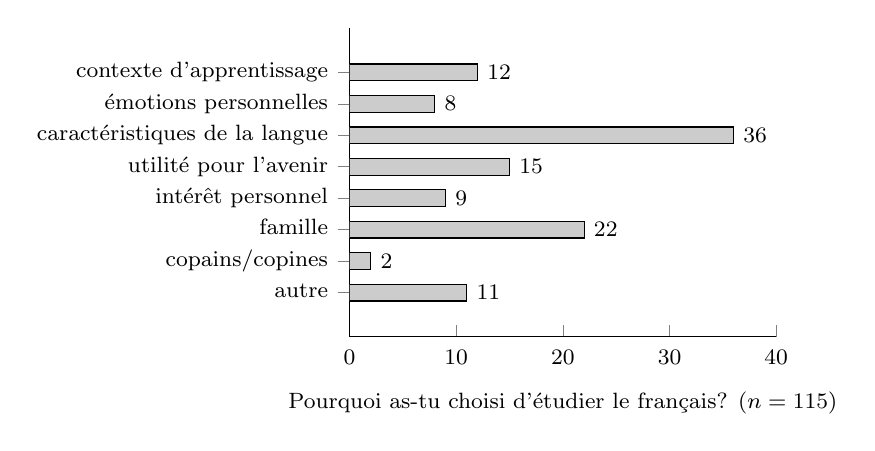
\begin{tikzpicture}
  \begin{axis}[
      xbar,
      axis lines*=left,
      bar width = 6pt,
      xmin = 0,
      xmax = 40,
      width = 7cm,
      height = 5.5cm,
      xlabel={Pourquoi as-tu choisi d'étudier le français? ($n=115$)},
      yticklabels = {
        autre,
        copains/copines,
        famille,
        intérêt personnel,
        utilité pour l'avenir,
        caractéristiques de la langue,
        émotions personnelles,
        contexte d'apprentissage
      },
      ytick = data,
      typeset ticklabels with strut,
%       yticklabel style={text width=8.5cm,align=right},
      tick label style={font=\footnotesize},
      nodes near coords,
      nodes near coords style={font=\footnotesize},
      nodes near coords align={horizontal},
      font=\footnotesize,
      enlarge y limits = 0.2
        ]
        \addplot [draw=black, fill=black!20] coordinates {
          (11,0)
          (2,1)
          (22,2)
          (9,3)
          (15,4)
          (36,5)
          (8,6)
          (12,7)
        };
  \end{axis}
  \end{tikzpicture}

\caption{\label{fig:granfeldt:4}Auto-évaluation des facteurs qui ont influencé les élèves à choisir le français: nombre de réponses au total. Les catégories d’analyse de la \figref{fig:granfeldt:4} proviennent de la littérature antérieure mentionnée dans le \sectref{sec:granfeldt:5.1} et incluent des réponses diverses : La mention du contexte d’apprentissage (le caractère du groupe, de l’enseignant ou d’autres élèves) ; des émotions personnelles (c’est amusant, chouette, intéressant, …) ; les caractéristiques de la langue (une belle/jolie langue) ; l’utilité pour l’avenir (besoin pour les études, la carrière, un futur métier, des voyages envisagés, etc.) ; un intérêt personnel (pour la France, Paris, la culture, l’histoire ou le film) ; la famille (l’influence des parents, des frères et sœurs ou des cousin(e)s).}
\end{figure}

La raison la plus souvent évoquée par les élèves est liée à une caractéristique de la langue elle-même : sa~beauté ($n=36$), comme exemplifié dans \REF{ex:granfeldt:1} : 

\ea%1
    \label{ex:granfeldt:1}
    Parce que je pense que c’est une langue extrêmement belle. 
\z

Bien que la plupart n’expliquent pas le caractère de cette beauté, certains mentionnent sa sonorité et sa mélodie. Le sentiment que la langue française est très belle semble répandu parmi les élèves du projet TAL. Un autre facteur central est l’influence de la famille, qui est mentionnée par 22 élèves. Les parents ou les frères et sœurs, comme illustré dans les exemples \REF{ex:granfeldt:2} et \REF{ex:granfeldt:3}, sont indiqués comme des sources d’inspiration mais aussi comme une aide dans les devoirs de français.

\ea%2
    \label{ex:granfeldt:2}
    Parce que ma mère et ma sœur ont étudié la langue et habité en France et elles pourront m’aider avec la langue.
\ex%3
    \label{ex:granfeldt:3}
    {[…]} l’un de mes frères a choisi le français et il m’a dit que c’était amusant.
\z

En revanche, nous pouvons constater que les amis sont très rarement mentionnés comme exerçant une influence directe sur le choix du français ($n=2$).

En outre, un groupe d’élèves ($n=12$) mentionne des facteurs très concrets liés à leur collège et au contexte scolaire dans lequel ils se trouvent. Comme dans l’exemple \REF{ex:granfeldt:4}, certains évoquent le fait que la classe de français est souvent plus petite que celle d’espagnol ou d’allemand, ce qui est ressenti comme un avantage. D’autres mentionnent une enseignante particulièrement populaire en FLE, comme illustré sous \REF{ex:granfeldt:5}. 

\ea%4
    \label{ex:granfeldt:4}
    {[J’ai]} choisi le français parce que j’avais entendu que la classe de français était petite et j’ai pensé alors qu’on peut avoir plus d’aide et qu’il est moins gênant de faire des présentations et de parler devant la classe. 
\ex%5
    \label{ex:granfeldt:5}
    Je l’ai choisi aussi parce qu’il y avait un si bon prof de français à la différence de l’espagnol. 
\z

Il est clair que pour certains élèves, des facteurs contextuels jouent un rôle primordial pour leur choix. Ce facteur est plus souvent commenté que celui d’un intérêt personnel particulier, comme la culture et l’histoire françaises, le film ou le sport ($n=8$).

Finalement, un quart des élèves ($n=15$) ont une vision claire de ce qu’ils veulent faire dans l’avenir et pour eux le français fait partie de leurs besoins futurs liés à des études, une carrière professionnelle ou encore des voyages après le bac. Dans toutes ces situations, il sera important de bien maîtriser la langue française et c’est pour cette raison qu’ils ont choisi d’étudier le français au collège, comme l’exprime un élève dans l’exemple \REF{ex:granfeldt:6}.~Il est conscient du fait que le français est une langue internationale qui peut donc être utile pour lui.

\ea%6
    \label{ex:granfeldt:6}
    Parce que c’est le mieux pour mon avenir. Dans les métiers qui m’intéressent, c’est un grand avantage de parler français. {[…]}. C’est aussi une belle langue qui est parlée dans beaucoup de pays du monde entier. 
\z

Ces élèves semblent avoir une vision de l’utilité du français dans leur avenir et se voient comme de futurs utilisateurs de la langue. Nous pouvons cependant noter que ces élèves ne sont pas en majorité dans notre échantillon, ce qui sera encore plus clair dans la sous-section suivante.

\subsubsection{L’utilité du français dans la vie quotidienne et future}

Il est impossible d’évoquer les attitudes des élèves suédois envers le FLE sans aussi mentionner leurs attitudes envers l’anglais. Comme dans la littérature antérieure \citep{Busse2017}, l’attitude positive envers l’anglais ressort également des données de notre questionnaire. Comme la \figref{fig:granfeldt:5} le montre, les réponses des élèves suédois, qui sont presque tous entièrement d’accord, confirment la position de l’anglais comme la langue la plus importante à apprendre. En revanche, la nécessité d’apprendre le français pour une personne qui parle déjà bien l’anglais est moindre, selon un grand nombre des élèves (voir \figref{fig:granfeldt:6}). Près de la moitié d’entre eux semblent d’accord ou presque d’accord (réponses 4 ou 5) sur le fait qu’une personne qui parle anglais n’a pas vraiment besoin d’apprendre le français.

\begin{figure}
% % % \includegraphics[width=\textwidth]{figures/granfeldt5.png}
  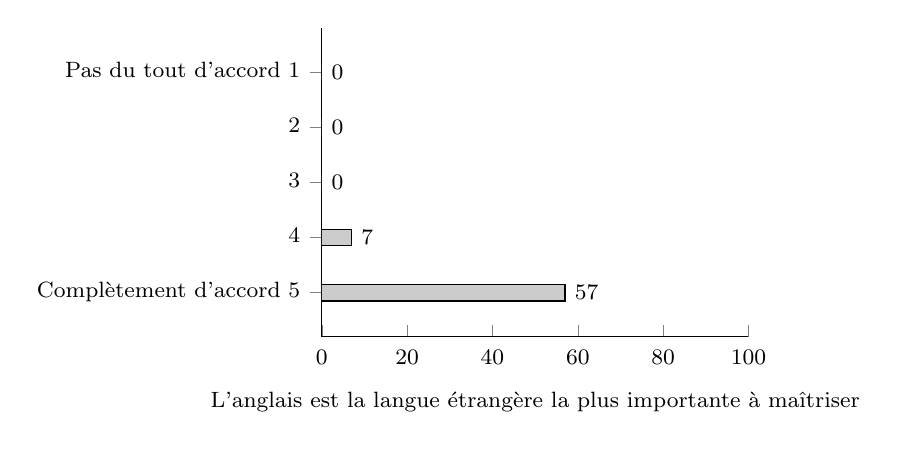
\begin{tikzpicture}
  \begin{axis}[
      xbar,
      axis lines*=left,
      bar width = 6pt,
      xmin = 0,
      xmax = 100,
      width = 7cm,
      height = 5.5cm,
      xlabel={L'anglais est la langue étrangère la plus importante à maîtriser},
      yticklabels = {%
        Complètement d'accord 5,
        4,
        3,
        2,
        Pas du tout d'accord 1
      },
      ytick = data,
      typeset ticklabels with strut,
%       yticklabel style={text width=8.5cm,align=right},
      tick label style={font=\footnotesize},
      nodes near coords,
      nodes near coords style={font=\footnotesize},
      nodes near coords align={horizontal},
      font=\footnotesize,
      enlarge y limits = 0.2
        ]
        \addplot [draw=black, fill=black!20] coordinates {
          (57,0)
          (7,1)
          (0,2)
          (0,3)
          (0,4)
        };
  \end{axis}
  \end{tikzpicture}
\caption{\label{fig:granfeldt:5}Les attitudes des élèves suédois envers l’anglais ($n=64$)}
\end{figure}
  
\begin{figure}
% % % \includegraphics[width=\textwidth]{figures/granfeldt6.png}
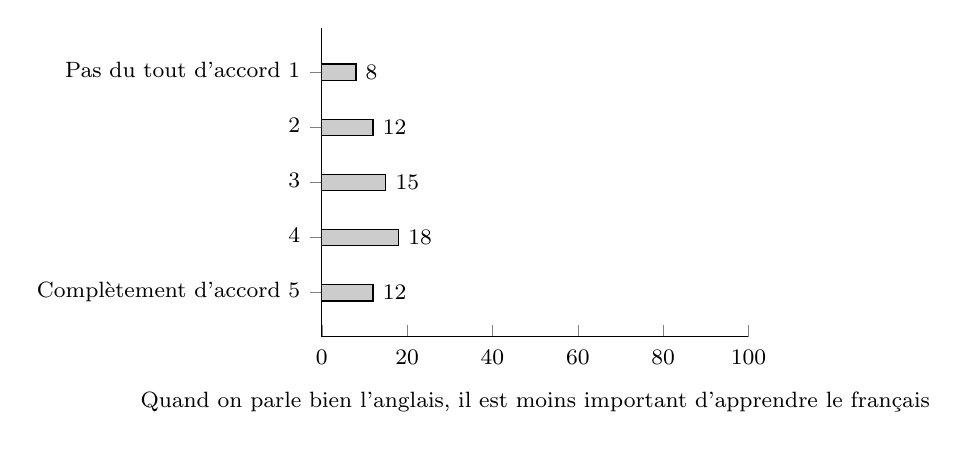
\begin{tikzpicture}
  \begin{axis}[
      xbar,
      axis lines*=left,
      bar width = 6pt,
      xmin = 0,
      xmax = 100,
      width = 7cm,
      height = 5.5cm,
      xlabel={Quand on parle bien l'anglais, il est moins important d'apprendre le français},
      yticklabels = {%
        Complètement d'accord 5,
        4,
        3,
        2,
        Pas du tout d'accord 1
      },
      ytick = data,
      typeset ticklabels with strut,
%       yticklabel style={text width=8.5cm,align=right},
      tick label style={font=\footnotesize},
      nodes near coords,
      nodes near coords style={font=\footnotesize},
      nodes near coords align={horizontal},
      font=\footnotesize,
      enlarge y limits = 0.2
        ]
        \addplot [draw=black, fill=black!20] coordinates {
          (12,0)
          (18,1)
          (15,2)
          (12,3)
          (8,4)
        };
  \end{axis}
  \end{tikzpicture}
\caption{\label{fig:granfeldt:6}Les attitudes des élèves suédois qui comparent le français avec l’anglais ($n=65$)}
\end{figure}

L’utilité, la nécessité et le caractère indispensable de l’anglais sont souvent mentionnés par les adolescents qui pensent à leurs futures études, leur carrière ou à leurs vacances et loisirs. Comme on l’observe dans les Figures 7 et 8, les opinions des élèves de FLE sur l’utilité du français pour leur avenir sont beaucoup moins unanimes. Peu d’élèves espèrent pouvoir utiliser le français dans leur vie quotidienne dans dix ans et les réponses sur l’utilité du français dans l’avenir sont mitigées. Autour de 35\% des élèves (réponses 4 ou 5) pensent que le français sera une ressource utile dans leur vie future. Les autres sont neutres (18\%) ou rejettent cette idée (46\%).

  
\begin{figure}
% % % \includegraphics[width=\textwidth]{figures/granfeldt7.png}
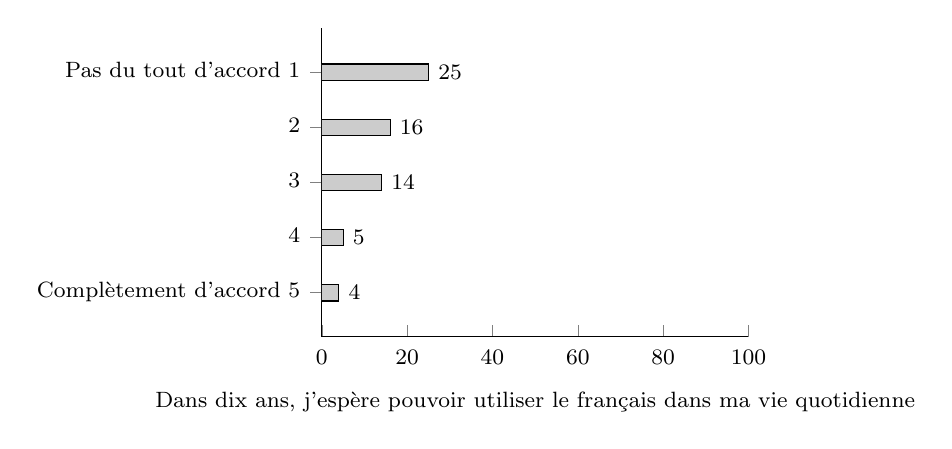
\begin{tikzpicture}
  \begin{axis}[
      xbar,
      axis lines*=left,
      bar width = 6pt,
      xmin = 0,
      xmax = 100,
      width = 7cm,
      height = 5.5cm,
      xlabel={Dans dix ans, j'espère pouvoir utiliser le français dans ma vie quotidienne},
      yticklabels = {%
        Complètement d'accord 5,
        4,
        3,
        2,
        Pas du tout d'accord 1
      },
      ytick = data,
      typeset ticklabels with strut,
%       yticklabel style={text width=8.5cm,align=right},
      tick label style={font=\footnotesize},
      nodes near coords,
      nodes near coords style={font=\footnotesize},
      nodes near coords align={horizontal},
      font=\footnotesize,
      enlarge y limits = 0.2
        ]
        \addplot [draw=black, fill=black!20] coordinates {
          (4,0)
          (5,1)
          (14,2)
          (16,3)
          (25,4)
        };
  \end{axis}
  \end{tikzpicture}
\caption{\label{fig:granfeldt:7}L’espoir d’un jour savoir parler français dans la vie quotidienne ($n=65$)}
\end{figure}
  
\begin{figure}
% % % \includegraphics[width=\textwidth]{figures/granfeldt8.png}
 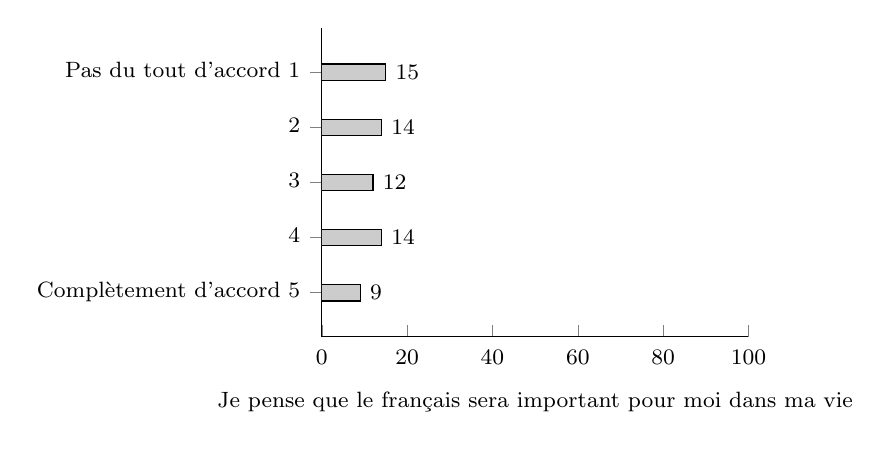
\begin{tikzpicture}
  \begin{axis}[
      xbar,
      axis lines*=left,
      bar width = 6pt,
      xmin = 0,
      xmax = 100,
      width = 7cm,
      height = 5.5cm,
      xlabel={Je pense que le français sera important pour moi dans ma vie},
      yticklabels = {%
        Complètement d'accord 5,
        4,
        3,
        2,
        Pas du tout d'accord 1
      },
      ytick = data,
      typeset ticklabels with strut,
%       yticklabel style={text width=8.5cm,align=right},
      tick label style={font=\footnotesize},
      nodes near coords,
      nodes near coords style={font=\footnotesize},
      nodes near coords align={horizontal},
      font=\footnotesize,
      enlarge y limits = 0.2
        ]
        \addplot [draw=black, fill=black!20] coordinates {
          (9,0)
          (14,1)
          (12,2)
          (14,3)
          (15,4)
        };
  \end{axis}
  \end{tikzpicture}
\caption{\label{fig:granfeldt:8}L’utilité du français dans l’avenir, selon les élèves suédois ($n=65$)}
\end{figure}

\subsubsection{Les leçons de français: quelles activités ?}

Un premier constat, basé sur les réponses libres des élèves à la question \textit{Quelles activités dominent les leçons de français ?} est qu’il y a forcément une variation dans les activités mentionnées.\footnote{{Au total les élèves en langues vivantes auront 340 heures d’enseignement (minimum) au collège dont au moins 48 heures en 6\textsuperscript{e} classe mais les établissements scolaires décident eux-mêmes la manière de distribuer le nombre d’heures par semaine et par an. Pour la plupart, il s’agit d’environ 2h à 2,5h d’enseignement de la langue vivante par semaine.}} Huit élèves soulignent explicitement cette variation dans l’enseignement dans leurs réponses, ce qui est aussi confirmé par le fait que 29 élèves énumèrent au moins trois activités habituelles, et parfois plus, pour caractériser les activités dans les leçons de FLE. En outre, le travail en classe semble très centré sur le manuel de français (livre de textes et cahier d’exercices). 25 élèves décrivent que leur manuel est le pivot de l’enseignement. Sachant que le manuel inclut à la fois des textes et des exercices de grammaire, de vocabulaire, de compréhension orale et écrite, des tâches de conversation et des jeux, il faut regarder les réponses plus en détail pour avoir de l’information sur les compétences qui sont travaillées en classe de français, selon les élèves. La distribution des réponses liées aux capacités spécifiquement entraînées en classe de français ($n=111$) se trouve résumée dans la \figref{fig:granfeldt:9}. Il faut noter que certains participants ont indiqué plusieurs capacités différentes, ce qui explique pourquoi nous référons ici~à 111 réponses au total pour les 65 participants.

  
\begin{figure}
% % % \includegraphics[width=\textwidth]{figures/granfeldt9.png}
 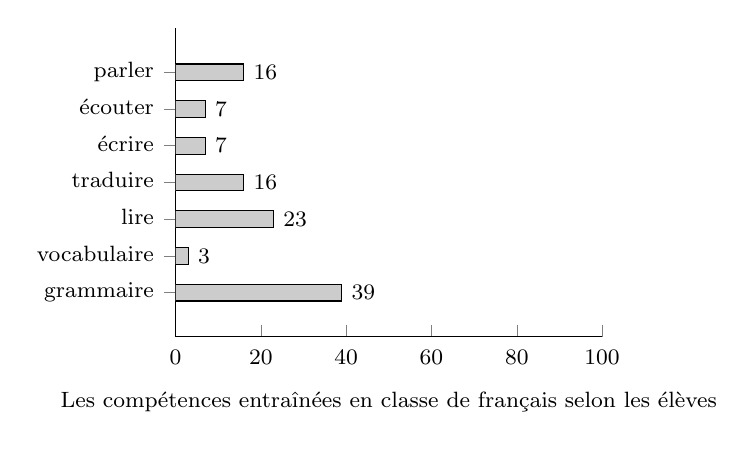
\begin{tikzpicture}
  \begin{axis}[
      xbar,
      axis lines*=left,
      bar width = 6pt,
      xmin = 0,
      xmax = 100,
      width = 7cm,
      height = 5.5cm,
      xlabel={Les compétences entraînées en classe de français selon les élèves},
      yticklabels = {%
        grammaire,
        vocabulaire,
        lire,
        traduire,
        écrire,
        écouter,
        parler
      },
      ytick = data,
      typeset ticklabels with strut,
%       yticklabel style={text width=8.5cm,align=right},
      tick label style={font=\footnotesize},
      nodes near coords,
      nodes near coords style={font=\footnotesize},
      nodes near coords align={horizontal},
      font=\footnotesize,
      enlarge y limits = 0.2
        ]
        \addplot [draw=black, fill=black!20] coordinates {
          (39,0)
          (3,1)
          (23,2)
          (16,3)
          (7,4)
          (7,5)
          (16,6)
        };
  \end{axis}
  \end{tikzpicture}
 

\caption{\label{fig:granfeldt:9}Les compétences travaillées en classe de français, selon les élèves suédois}
\end{figure}

Selon un grand nombre d’élèves ($n=39$), c’est la grammaire qui se trouve au centre des activités dans les classes de français. Certains élèves, comme dans l’exemple \REF{ex:granfeldt:7}, ne mentionnent que cette activité alors que d’autres, comme dans l’exemple \REF{ex:granfeldt:8}, décrivent que la grammaire est une partie importante de l’enseignement qui intègre aussi d’autres activités.

\ea%7
    \label{ex:granfeldt:7}
    Nous parlons beaucoup de la grammaire~et de quand il faut l’utiliser.
\z

\ea%8
    \label{ex:granfeldt:8}
    Nous avons beaucoup de présentations de grammaire et nous faisons aussi beaucoup d’exercices qui y sont liés. C’est probablement ce que nous faisons le plus souvent mais nous travaillons aussi durement avec la lecture et la traduction des textes français~de notre manuel. 
\z

Nous pouvons y ajouter que quatre élèves spécifient que ce sont «~les verbes~» qui se trouvent au centre des activités de grammaire. En comparaison, le vocabulaire n’est mentionné que par trois élèves. 

De plus, la traduction de textes accompagne souvent les activités grammaticales. Comme illustré dans l’exemple \REF{ex:granfeldt:9}, un groupe d’élèves ($n=17$) précise que la traduction est une activité importante, souvent intégrée dans le travail avec le manuel de français.

\ea%9
    \label{ex:granfeldt:9}
    Nous travaillons le plus souvent avec les textes que nous traduisons puis nous faisons des exercices qui y sont liés. Il y a souvent de la grammaire aussi. 
\z

Si nous y ajoutons les commentaires qui mentionnent la lecture ou la compréhension écrite ($n=23$) et la rédaction de textes et la production écrite ($n=7$), nous constatons que les élèves semblent passer une grande partie du temps en classe de français à travailler la langue écrite et les structures de la langue dans des activités de grammaire et de traduction liées aux manuels.

\begin{sloppypar}
En contraste, relativement peu d’élèves mentionnent les activités qui intègrent la langue parlée. Sept élèves évoquent les exercices de compréhension orale et seize élèves mettent en avant la production orale («~parler~») ou l’interaction («~discuter~») avec les membres de la classe. Dans l’exemple \REF{ex:granfeldt:10}, un élève constate~que les activités orales sont plutôt rares~dans ses cours de FLE.
\end{sloppypar}

\ea%10
    \label{ex:granfeldt:10}
    {[…]} parfois nous lisons à haute voix mais c’est rare que nous parlions oralement les uns avec les autres. 
\z

Après avoir décrit les activités dans les cours de FLE, mentionnées par les élèves, nous allons maintenant tourner le regard vers leurs attitudes et leurs émotions par rapport à ces activités. 

\subsubsection{Les attitudes des élèves envers les activités en classe de FLE}

Les réponses à la question ouverte \textit{Qu’est-ce qui est amusant aux cours de FLE et que-ce qui est moins amusant ?} nous donnent quelques indications intéressantes sur les attitudes des élèves. Tout d’abord, une vingtaine d’élèves ne mentionnent pas d’activités précises mais se contentent à constater que «~tout me plaît~», «~je déteste le français~» ou sinon «~je n’aime pas les devoirs~», etc. D’autres élèves sont plus informatifs quant à leurs attitudes envers des activités spécifiques en classe. Parmi les activités les plus appréciées, nous trouvons les exercices oraux : parler et interagir avec les pairs en français ($n=15$), comme illustré dans l’exemple \REF{ex:granfeldt:11}, ou sinon écouter et essayer de comprendre ce qu’on dit ($n=7$) (voir \citealt{BusseWilliams2010, Oakes2013}). 

\ea%11
    \label{ex:granfeldt:11}
    Je trouve que le plus amusant c’est de parler et de faire la conversation avec les autres dans la classe de français. Mais je trouve ennuyeux de travailler la grammaire.
\z

Or, les activités liées à la langue écrite sont aussi mentionnées~par un nombre d’élèves qui apprécient la lecture de textes en français ($n=8$) et la rédaction de textes ($n=5$). Certains mentionnent aussi qu’ils aiment apprendre du vocabulaire et des expressions utiles ($n=6$) et travailler la grammaire ($n=4$). L’attitude négative envers les exercices de grammaire, signalé dans l’exemple \REF{ex:granfeldt:11}, ressort pourtant clairement des réponses sur les activités que les élèves n’apprécient pas ($n=17$). D’autres mentionnent le travail dans le manuel ($n=4$), la lecture et la traduction ($n=4$) comme étant des activités moins appréciées. En effet, plusieurs élèves expriment le contraste entre les activités orales et le travail avec les exercices de grammaire qui sont laborieux selon certains et ennuyeux selon d’autres. L’exemple \REF{ex:granfeldt:12} illustre cette dichotomie avec quelques nuances.

\ea%12
    \label{ex:granfeldt:12}
    C’est amusant quand on comprend ce que dit le professeur ou quand on comprend complètement un texte et quand on peut parler avec quelqu’un. C’est moins drôle avec la grammaire parce qu’on n’y comprend rien !
\z

Il faut pourtant aussi mentionner qu’un petit groupe d’élèves ($n=4$) mentionnent des difficultés ressenties avec les exercices oraux qui sont liées aux émotions négatives et le stress lorsqu’il faut parler devant la classe (cf. \textit{second language anxiety}, \citealt{HorwitzEtAl1986}), comme illustré dans l’exemple \REF{ex:granfeldt:13}.

\ea%13
    \label{ex:granfeldt:13}
    Je trouve que c’est moins amusant de parler devant la classe puisque je trouve cela très dur et je me sens toujours nerveux.
\z

Pour terminer, mentionnons aussi les commentaires libres à la fin du questionnaire, où les élèves ont eu la possibilité d’ajouter encore des réflexions personnelles s’ils en ressentaient besoin. Certains élèves, dont celui qui s’exprime dans l’exemple \REF{ex:granfeldt:14}, ont alors saisi l’occasion d’élaborer encore leurs avis sur l’enseignement de français. 

\ea%14
    \label{ex:granfeldt:14}
    Je veux parler plus ! À la fois en français et en anglais. Je trouve que c’est surtout cela qui sera utile dans l’avenir. 
\z

\begin{sloppypar}
Ce commentaire accentue encore un déséquilibre vécu par certains élèves entre les activités qui dominent dans la salle de classe de français (grammaire, traduction, textes…), d’un côté, et les outils communicatifs pour l’avenir (parler, communiquer, discuter), de l’autre côté. Ce sont ces derniers qui, pour un groupe important d’élèves, correspondent aux activités les plus appréciées et les compétences qu’ils souhaitent maitriser dans l’avenir.
\end{sloppypar}

\section{Discussion}\label{sec:granfeldt:6}

\subsection{Anna: Apprenante guidée du FLE en Suède}\label{sec:granfeldt:6.1}

Parmi les nombreux élèves que nous avons rencontrés lors du projet TAL, il y a Anna, une adolescente de 15 ans, qui habite dans une petite commune dans le nord de la Suède avec 18.000 habitants, dont 6.000 dans la ville-centre. Au moment où nous avons rencontré Anna, elle étudiait le FLE depuis trois ans. Elle avait choisi le FLE parce qu’elle trouvait que le français était une belle langue et parce qu’elle avait envie d’aller un jour en France. Le choix du français était entièrement le sien et depuis toujours elle avait cette envie d’apprendre le français. Anna aime bien lire et écouter des émissions en français et adore le défi d’essayer de comprendre ce qu’on dit. De manière générale, Anna aime les langues et elle voudrait en apprendre plusieurs dans sa vie. Elle considère que l’anglais est la langue étrangère la plus importante pour elle, mais elle dit être fière d’apprendre le français et aime que les autres la considèrent comme une personne qui connaît cette langue. Pourtant, elle ne pense pas que le français jouera un rôle important dans sa vie quotidienne dans l’avenir. L’établissement scolaire d’Anna est un collège, le plus grand des quatre collèges de la commune, et intègre environ 350 élèves en 2021. En 2000, quinze pour cent des élèves qui avaient choisi une langue vivante dans la commune avaient choisi le FLE. Ces dernières années (2020--2021), ce chiffre oscille entre deux et six pour cent. Lors de notre visite en 2018, le principal de l’établissement nous a affirmé que depuis quelques années son collège était le seul de la commune à offrir le FLE et qu’il y a déjà eu plusieurs discussions dans le passé pour enlever le FLE du programme même de ce collège parce que le nombre d’élèves qui choisissent le FLE était insuffisant. Le coût élevé de ces petits groupes d’enseignement constitue souvent un problème économique pour l’établissement scolaire et le principal ne peut pas garantir que le FLE y soit toujours une option dans l’avenir. Dans la classe de français d’Anna, il y avait au moment de notre visite six élèves.\largerpage

Le fait qu’Anna ait appris le FLE dans une petite ville dans le nord de la Suède est le résultat de toute une série de circonstances et de choix à différents niveaux. L’apprenante que nous avons nommée Anna se trouve au cœur d’un écosystème éducatif complexe qui définit largement les conditions de son apprentissage des langues vivantes. Dans cette contribution, un premier objectif a été de discuter certaines de ces conditions et leurs effets pour l’enseignement du FLE en Suède à l’aide d’un modèle à trois niveaux~(\citealt{TheDouglasFirgroup2016}) : \textit{macro, méso} et \textit{micro}. Au niveau \textit{macro}, la politique linguistique éducative du pays a eu pour résultat une politique d’accès (\citealt{KaplanBaldauf2005}) à une langue vivante après l’anglais construite autour des valeurs du choix et de la concurrence qui sont à la base du système éducatif suédois depuis les années 1990 (\citealt{YangHansenGustafsson2016}). Alors qu’il a été obligatoire pour Anna de faire un choix linguistique en plus de l’anglais, il a été facultatif de choisir une langue vivante telle que le FLE. Toujours au niveau \textit{macro}, la politique linguistique a pourtant privilégié trois langues étrangères, le FLE, l’ALE et l’ELE qui ont un statut spécifique ; deux de ces trois langues doivent être proposées par les communes et les organisateurs indépendants (\citealt{Ministèredéducation2011}). Avec son rêve depuis toujours d’apprendre le FLE, Anna a eu la chance d’être née dans une commune et d’habiter près d’un collège qui, à l’époque, proposait le FLE au programme des langues vivantes. Il n’est pas certain que ce choix existe encore d’ici quelques années. Le fait qu’elle avait choisi le FLE et non pas l’ALE ou l’ELE semble être le résultat d’une attitude globale et stéréotypée vis-à-vis du français, celle d’une beauté particulière de la langue. Pourtant, à la différence de l’anglais, le FLE ne semble pas faire partie de ses projets individuels pour l’avenir.

\subsection{L’avenir du FLE en Suède: Tendances positives et négatives}\label{sec:granfeldt:6.2}\largerpage

Un deuxième objectif de cette contribution a été de tracer le développement du FLE en Suède depuis l’entrée du pays dans l’UE et d’essayer d’envisager son avenir. En ce qui concerne le développement pendant ces 25 dernières années, nos analyses aux niveaux \textit{macro} et \textit{méso} ont montré quelques tendances claires. Après une première période pendant laquelle le FLE a perdu des élèves au profit de l’ELE, le niveau s’est stabilisé autour de quinze pour cent des élèves après 2007, l’année de l’introduction des points supplémentaires pour les études de langues vivantes. Avec \citet{Spolsky2004}, on peut alors conclure que cette mesure de gestion a eu l’effet souhaité au niveau des pratiques des jeunes mais la question reste ouverte en ce qui concerne les croyances. Les attitudes enregistrées des élèves ne semblent pas s’aligner avec l’idée d’une utilité du FLE pour l’avenir. En plus, la stabilisation du FLE ne concerne pas le pays entier. Nous avons pu constater que parmi les trois langues vivantes principales, l’offre de FLE s’est réduite de façon importante pendant la même période, surtout dans les petites communes. Bien qu’une proportion d’élèves stable au niveau national fasse des études de FLE en 2022, le nombre de communes dans lesquelles il n’y a plus d’élèves de FLE est cinq fois plus élevé qu’en 2007.

En ce qui concerne la question de l’avenir du FLE dans le contexte scolaire en Suède, ce sont dans ces tendances qu’il faut chercher les éléments d’une réponse possible. D’abord on peut constater qu’il y a des tendances positives. Au niveau \textit{macro}, la politique linguistique éducative a changé en 2007 sous l’effet de l’introduction d’une «~carotte~» constituée de points supplémentaires pour les élèves ayant étudié des langues vivantes à des niveaux avancés au lycée. D’après nos analyses, il est probable que cette mesure a eu un effet positif sur la proportion d’élèves au collège qui décident d’étudier une langue vivante. Par rapport au FLE, l’effet a été positif parce qu’une grande partie des élèves de FLE provient d’une classe sociale où il est normal de faire des études supérieures, habitant surtout dans les villes universitaires, les grandes villes ou les communes proches des grandes villes. En d’autres termes, cette mesure a ciblé un public parmi lequel le choix du FLE était déjà une tradition. 

En même temps, il y a aussi des tendances négatives pour le FLE qui illustrent la complexité et l’interdépendance des niveaux différents du modèle. Le cas le plus clair concerne la décision récente prise en 2018 de ne plus laisser aux communes le choix de commencer l’enseignement des langues vivantes en 6\textsuperscript{e} (12 ans) ou en 7\textsuperscript{e} (13 ans) classe. Cette décision au niveau \textit{macro} (politique linguistique éducative) est basée sur la conviction qu’un début d’apprentissage plus précoce conduira à de meilleurs résultats. Nos analyses montrent qu’il est probable que cette décision ait déjà entraîné des conséquences négatives au niveau \textit{méso}, notamment en ce qui concerne l’offre de FLE à travers le pays. En fait, le nombre des communes qui n’enregistrent pas d’élèves de FLE a augmenté de 40 à 50 depuis cette décision. Cette évolution pourrait être le début d’un cercle vicieux pour le FLE dont les conséquences seront encore plus visibles dans l’avenir. Avec une réduction de l’offre de FLE, il y aura moins de membres de famille, moins de frères et sœurs et, à plus long terme, moins de parents qui auront étudié le FLE au collège et au lycée et ainsi moins d’apprenants modèles vers qui les futurs élèves pourront se tourner au moment de leur choix d’une langue vivante. Nos analyses des questionnaires au niveau \textit{micro} montrent que les membres de famille sont importants dans le processus du choix. Les expériences des membres de la famille proche en tant qu’apprenants d’une langue vivante spécifique représentent une source d’information unique et importante. De façon inverse, on peut parler d’un cercle vertueux pour l’ELE. Après son introduction en 1994, il y a de plus en plus d’élèves et ainsi de membres de famille et de camarades qui ont appris la langue, ce qui a eu pour résultat que cette langue aujourd’hui est enseignée dans pratiquement tous les établissements scolaires en Suède. 

Au cœur de ces tendances se trouvent, toujours au niveau \textit{micro}, les attitudes et les motivations des élèves par rapport au FLE. A la différence de l’anglais, langue associée à une très grande utilité et nécessité pour réaliser des projets personnels, le FLE est souvent choisi sur la base d’une appréciation globale en tant que langue («~le français est une très belle langue~»). Qui plus est, la perception de l’enseignement qu’ont les élèves ne semble pas les aider à développer d’autres images liées au FLE. Les élèves expriment que, selon eux, c’est avant tout la compétence grammaticale, la traduction et les textes qui sont travaillés dans la classe de langue.~Même si cette perception ne serait pas objectivement correcte, elle représente un problème dans la mesure où elle empêche les élèves de développer leur confiance en eux en tant que locuteurs qui savent parler et interagir dans la langue cible, ce qui constitue, selon une majorité d’entre eux, leur besoin central pour l’avenir (\citealt{BusseWilliams2010, Oakes2013}). En revanche, c’est aussi à ce niveau \textit{micro} que se trouve la clé d’un changement possible. Sans le soutien des jeunes, la politique linguistique éducative du niveau \textit{macro} a beau privilégier l’apprentissage des langues vivantes en général et du FLE en particulier (\citealt{Mitchell2009}), ce sont les choix, la détermination et l’investissement des élèves qui décideront en dernier lieu de l’avenir du FLE en Suède, un constat qui n’est d’ailleurs en rien spécifique à ce pays.

\section{Conclusion}\label{sec:granfeldt:7}

L’apprenant guidé d’une langue étrangère se trouve au cœur d’un écosystème éducatif complexe qui détermine largement ses possibilités d’apprentissage et les résultats de son acquisition. Dans les recherches, il y a un consensus émergeant que face à cette complexité il faudra mettre en dialogue différentes disciplines afin d’arriver à discuter l’apprentissage des langues dans toute sa complexité. S’il existe déjà des approches écologiques de l’apprentissage des langues secondes et étrangères, le modèle du \citet{TheDouglasFirgroup2016} propose un cadre transdisciplinaire intégrant, entre autres, les sciences de l’éducation, la sociologie, les sciences cognitives, la psychologie et la linguistique, pour l’étude de ces questions aux niveaux \textit{macro, méso} et \textit{micro}.

Dans cette contribution, nous nous sommes donné deux objectifs. Le premier consistait à essayer d’appliquer ce modèle sur la situation du FLE en Suède, ce qui nous a permis de tracer comment les idéologies linguistiques sur le plan national ont été implémentées dans les politiques linguistiques éducatives avec des effets sur la proportion d’élèves qui étudie le FLE et sur l’offre de FLE au niveau des établissements scolaires à travers le pays. Le modèle nous a également permis d’étudier les facteurs susceptibles de déterminer le choix des élèves du FLE comme langue vivante à l’école et leurs émotions et attitudes envers la langue française et les activités qui dominent en classe de FLE. 

Le deuxième objectif a été de tracer le développement du FLE dans le contexte scolaire depuis l’entrée de la Suède dans l’Union européenne et de discuter de son avenir. Alors qu’il y a eu pendant cette période des mesures qui ont eu des effets positifs sur la proportion d’élèves choisissant le FLE, notamment l’introduction des points supplémentaires pour les cours de langues vivantes, il y a aussi des tendances négatives. A la différence des deux autres langues vivantes principales, à savoir l’allemand et l’espagnol, le FLE est en train de disparaître de l’offre éducative d’un nombre grandissant de collèges. Nos analyses suggèrent que ce développement est actuellement accéléré par la décision prise au niveau \textit{macro} en 2018 d’obliger les établissements scolaires de commencer l’enseignement des langues vivantes au plus tard en 6\textsuperscript{e} classe. Cette décision politique, fondée sur l’observation qu’il vaut mieux commencer l’apprentissage d’une nouvelle langue le plus tôt possible, était une mesure prise dans l’optique de renforcer la place des langues vivantes à l’école. Paradoxalement, pour des raisons administratives et économiques, il semble que cette même mesure ait ouvert la voie à une diminution du nombre de langues vivantes proposées dans les établissements scolaires. Cette tendance, qui frappe avant tout le FLE, illustre parfaitement la complexité inhérente à ces questions.

\section*{Remerciements} 

En travaillant sur cette contribution, nous avons eu l’occasion de réfléchir aux travaux de Daniel et à ce qu’ils représentent pour nous. Avec une carrière si riche et active que la sienne, il est, bien évidemment, impossible d’en rendre compte en quelques lignes. S’il faut cependant choisir une qualité, qui caractérise non seulement ses travaux mais aussi la personne telle que nous la connaissons, ce serait son ouverture d’esprit. Cela tombe bien parce que c’est un SN, une structure syntaxique à laquelle Daniel a consacré beaucoup de temps et d’énergie, mais surtout parce que le sens véhiculé par cette expression reflète pour nous son intérêt et son respect des idées des autres, ce qu’il a souvent combiné avec une envie de réunir en dépassant les disciplines. C’est également cette qualité qui a inspiré la thématique de notre contribution. A tout cela s’ajoute, sur un plan plus personnel, une gentillesse et une bienveillance exceptionnelles que nous avons pu apprécier à maintes reprises et dont nous tenons à le remercier. Merci Daniel.

\printbibliography[heading=subbibliography,notkeyword=this]
\end{otherlanguage}
\end{document} 
